\documentclass[12pt,a4paper,english
% ,twoside,openright
]{tunithesis}

% Note that you must choose either Finnish or English here and there in this
% file.
% Other options for document class
  % ,twoside,openright   % If printing on both sides (>80 pages)
  % ,twocolumn           % Can be used in lab reports, not in theses

% Ensure the correct Pdf size (not needed in all environments)
\special{papersize=210mm,297mm}


% LaTeX file for BSC/MSc theses and lab reports.
% Requires the class file (=template) tunithesis.cls and figure files,
% either tut-logo, exampleFig (as pdf or eps) and example_code.c
% Author: Lucas Machado (2018)
% Based on TTU template by Sami Paavilainen (2006), modified by Heikki Huttunen (2014)

% More information about Latex basics:
% [Tobias Oetiker, Hubert Partl, Irene Hyna, Elisabeth Schlegl, The
% Not So Short Introduction to LATEX2e, Version 5.03, April 2014, 171
% pages.  Availbale: http://tobi.oetiker.ch/lshort/lshort.pdf]

\author{Väinö-Waltteri Granat}
\title{Zero to DLA: Building Software Support For Custom RISCV SoC To Run Complex Neural Networks} % primary title (for front page)
\thesistype{Master's thesis} % or Bachelor of Science, Laboratory Report... 

% Put your thesis' main language last
% http://mirrors.ctan.org/macros/latex/required/babel/base/babel.pdf
\usepackage{lastpage}
\usepackage[english]{babel}
\usepackage[
backend=biber,
style=numeric-comp,
citestyle=numeric-comp,
autocite=footnote
]{biblatex}
\usepackage{csquotes}
\usepackage{booktabs}
\usepackage{adjustbox}
\usepackage{subcaption}
\usepackage[withpage]{acronym}
\usepackage{tikz}
\usetikzlibrary{arrows.meta, arrows}
\usetikzlibrary{matrix}
\usepackage{xcolor}

\addbibresource{thesis_refs.bib} %Imports bibliography file

% Fix this
\newcommand{\fixthis}[1]{\textbf{\textit{\textcolor{red}{[#1]}}}}

\definecolor{tunipurple}{RGB}{78, 0, 142}

\newcommand\todo[1]{{\color{red}!!!TODO: #1}} % Remark text in braces appears in red
\newcommand{\angs}{\textsl{\AA}}              % , e.g. slanted symbol for Ångstöm

\pagenumbering{roman} % was: {Roman}
\pagestyle{headings}
\begin{document}

% Special trick so that internal macros (denoted with @ in their name)
% can be used outside the cls file (e.g. \@author)
\makeatletter

\thispagestyle{empty}
\vspace*{-.5cm}\noindent

\begin{figure}
    \vspace{-1.3cm}
    \advance\leftskip-2.5cm
    \noindent
\includegraphics{img/tunilogo.png}
\end{figure}
 
\vspace{2.5cm}
\begin{flushright}
\noindent\textsf{\LARGE{\@author}}

\noindent\vspace{0.5cm}

\noindent\Huge{\textsf{\textbf{\textcolor{tunipurple}{\@title}}}}
\end{flushright}
\vspace{10.7cm} % adjust to 12.7 this if thesis title needs two lines

% Last some additional info to the bottom-right corner
\begin{flushright}  
    \begin{spacing}{1.0}
      \textsf{Faculty of Information Technology and Communication Sciences (ITC)\\
      \@thesistype\\
      December 2024}
    \end{spacing}
\end{flushright}

% Leave the backside of title page empty in twoside mode
\if@twoside
\clearpage
\fi

% Turn off page numbering for the first pages
\pagenumbering{gobble}

\chapter*{Abstract}

\begin{spacing}{1.0}
\noindent \@author: \@title\\
\@thesistype\\
Tampere University\\
Master’s Degree Programme in Signal Processing and Machine Learning\\
December 2024
\end{spacing}
\noindent\rule{12cm}{0.4pt}

\vspace{0.5cm}

% ---------------------------------------
% Abstract and keywords
% ---------------------------------------

\noindent Lorem ipsum~

\noindent\textbf{Keywords:} DLA, Deep-Learning, SoC, Virtual Prototype.

~

\noindent The originality of this thesis has been checked using the Turnitin Originality Check service.


\clearpage

\section*{List of Abbreviations}
\begin{acronym}
  \acro{DLA}{Deep Learning Accelerator}
  \acro{DLA-VP}{Headsail Deep Learning Accelerator Virtual Prototype}
  \acro{SoC}{System on a chip}
  \acro{ISA}{Instruction set architecture}
  \acro{ML}{Machine Learning}
  \acro{AI}{Artifical Intelligence}
  \acro{DL}{Deep Learning}
  \acro{MPL}{Multilayer Perceptron}
  \acro{RGB}{Red Green Blue}
  \acro{DNN}{Deep Neural Network}
  \acro{CNN}{Convolutional Neural Network}
  \acro{CHW}{Channel Height Width}
  \acro{HWC}{Height Width Channel}
\end{acronym}



\setcounter{tocdepth}{3}              % How many header level are included
\tableofcontents                      % Create TOC

% The actual text begins here and page numbering changes to 1,2...
% Leave the backside of title empty in twoside mode
\if@twoside
%\newpage
\cleardoublepage
\fi


\renewcommand{\chaptername}{} % This disables the prefix 'Chapter' or
                              % 'Luku' in page headers (in 'twoside'
                              % mode)


\chapter{Introduction}
\label{ch:introduction}
\pagenumbering{arabic}
\setcounter{page}{1} % Start numbering from zero because command
                     % 'chapter*' does page break

In recent years neural network based application have become more and more prominent in our everyday-life. The large driver for this has been the adoption of efficient accelerators in mobile device, that have enabled running neural network applications of mobile devices, such as smart phones.

This interest in neural networks has coincided with the industry's move to heterogenous System-on-chip solutions being used in consumer and professional devices, to imporove computational performance.
More often these companies integrate their accelerators into SoCs, which include CPUs, GPUs, memory and other accelerators and peripherals in one package. Apple and Qualcomm have proved with their SoCs that they can attain desktop like performance in a smaller package than was previously possible. The industry moving towards SoCs has generated new interest in developing open-source SoCs.

The goal of this project was to build software support for the Deep-Learning Accelerator in the upcoming Headsail SoC from SocHub using a Renode based virtual prototype as the development platform. The goal was to use this concurrent development approach to have software support ready before the chip had been manufactured.

\chapter{Background}
This section covers the necessary knowledge in topics in Deep Learning that are needed to understand the development of the DLA software.
\label{ch:background}
\section{Machine Learning and Deep Learning}
Machine Learning is a field of computer science that researches algorithms to categorize data into distinct concepts so that yet unseen data can be categorized similarly. The central component of ML is always a model. Model is a function that distinguishes a concept from data.
To build a model we first need training data. Training data is a set of data, often with known associated categories, that corresponds with the unseen data we want to categorize with the model. For example if training a model to count the number of people in image, we would have a training data consisting of images with different amount of people, with the wanted categorization (number of people present in the image) associated with each.
Model is then trained by choosing a particular function and changing it's parameters so that it can categorize training data in a wanted manner. After training the performance can then be validated by feeding the model unseen data and seeing how well it can categorize it.
Turns out that some problems are hard to describe mathematically, and therefore finding a good function for modeling a problem might be nearly impossible in some cases. For example going back to the counting people in a picture describe, how do you event tell a computer what a person looks like?

It turns out that instead of carefully building a mathematical model it's easier to discover it. This is where artificial neural networks come in place. Neural networks are behind most bleeding edge advances in fields such as computer vision, image generation, AI chatbots and autonomous decision making systems.

Deep Learning is a subset of Machine Learning which focuses on multilayer perceptrons, neural networks with more than one hidden layer.
The goal of each DNN is to approximate a particular function.
In mathematics a function describes the relation between a domain $A$ and codomain $B$ where
\begin{equation}
  f \subseteq A \times B,
\end{equation}
meaning that for every element in the domain $A$ there is exactly one corresponding element in codomain $B$.

Intuitively domain $A$ can be viewed as the input of a multilayer perceptron and codomain $B$ as the output of the network. For a binary classifier codomain $B$ would be defined as
\begin{equation}
  B = \{0, 1\},
\end{equation}

and for 10 class classifier
\begin{equation}
  B = \{0, 1, 2 ..., 9\}.
\end{equation}
The domain of the network depends on the problem statement. For example for a image classifier the input can be viewed as a 3 dimensional array, where the second and third dimensions correspond to the height and width of the image and the first dimension as the channel in RGB color space as shown in figure~\ref{fig:rgb-array}, this commonly known as CHW layout.


\begin{figure}
  \centering
  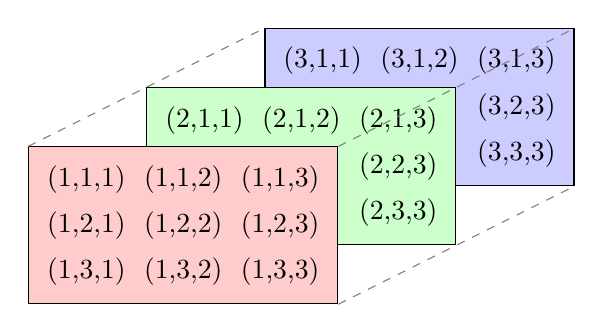
\begin{tikzpicture}
  \def\xs{-1.5} %shift in x direction
  \def\ys{-0.75} %shift in y direction
  \def\nm{3} % number of 2d matrices in the 3d matrix
  \foreach \x in {3,2,1}
  {
      \pgfmathsetmacro\bgcolor{ifthenelse(\x==1,"red!20",ifthenelse(\x==2,"green!20","blue!20"))}

      \matrix [draw, % for the rectangle border
              fill=\bgcolor, % different background colors
              ampersand replacement=\&] % see explanation
      (mm\x)% give the matrix a name
      at(-\x * \xs, -\x * \ys) % shift the matrix
      {
          \node {(\x,1,1)}; \& \node {(\x,1,2)}; \& \node {(\x,1,3)};\\
          \node {(\x,2,1)}; \& \node {(\x,2,2)}; \& \node {(\x,2,3)};\\
          \node {(\x,3,1)}; \& \node {(\x,3,2)}; \& \node {(\x,3,3)};\\
      };
  }

  \draw [dashed,gray](mm1.north west) -- (mm\nm.north west);
  \draw [dashed,gray](mm1.north east) -- (mm\nm.north east);
  \draw [dashed,gray](mm1.south east) -- (mm\nm.south east);
  \end{tikzpicture}
  \caption{RGB array}
  \label{fig:rgb-array}
\end{figure}

The purpose of the neural networks is map the values of array to the codomain in such a manner that useful information can be acquired from the mapping.
Now that we know the domain and the codomain of our DNN we need to discover a function that represents the relation between them.

\subsection{Convolutional Neural Networks}
Convolutional neural networks are a type of neural networks that heavily utilize convolution operations. Convolution is a useful operations used to extract features from data.


\subsection{Convolution}
Convolution is defined as
\begin{align}
  (f \ast g)(t) = \int_{-\infty}^{\infty}f(t-x)g(t)dx,
\end{align}
where $f$ and $g$ are functions to be convolved. For computer science the discrete convolution is often more interesting
\begin{align}
  (f \ast g)(i) = \sum_{m}f(i-m)g(m).
\end{align}
For DNNs we often think about convolution in terms of inputs($f$) and kernels($g$), where input is the useful data we want to extract features from and kernels are the specific selected values that can extract the wanted features from data.

When working with images, for example in a neural network used for classifying objects in images, it  natural to use the two dimensional expansion of the convolution operation
\begin{align}
  Conv2D(i, j) = (K \star I)(i,j) = \sum_{m}\sum_{n}I(i-m,j-n)K(m, n)
\end{align}
where $I$ is the input and $K$ is one kernel, $m$ is the width of the kernel and $n$ is the height.

In neural networks convolution is often implemented as cross-correlation but still called convolution, this is also what we have done in our implementation
\begin{align}
  Conv2D(i,j) = CrossCorrelation(I, K) = (K \star I)(i,j) = \sum_{m}\sum_{n}I(i+m,j+n)K(m, n)
\end{align}
To produce output of one layer one needs to calculate $Conv2D$ for all the positions in the resultant output matrix for all the kernels.

\subsection{Bias}
In addition to $Conv2d$ bias is another important concept in neural networks. Bias is a constant value applied to output channel of the preceding operation. In CNNs when applied after $Conv2d$ the purpose of bias is to signify the importance of each extracted feature. If bias is small or negative it means that the feature is non important for the particular class it's being applied. If bias is large or positive it means that the feature is important.

In mathematic notation bias is defined as such
\begin{align}
  y = xA^{T} + b
\end{align}
where if $xA^{T}$ is the non-biased output of a particular channel in layer, $b$ is the bias applied to the whole channel as a constant value.

\subsection{Activation function}
The combination of convolution and bias form one example of an affine transformation, a linear transformation between two space.
To enable neural networks to recognize non-linear features, we need to introduce non linear operations between the linear affine transformations. Traditionally we used sigmoid or tanh functions, which are defined as

\begin{align}
  \sigma(x) = \frac{1}{1+e^{-x}}
\end{align}
and,
\begin{align}
  tanh(x) = \frac{e^{x}-e^{-x}}{e^{x}-e^{-x}},
\end{align}
to introduce non-linearity. Both functions suffer from the fact that they are expensive to calculate and exhibit the vanishing gradient problem.~\parencite{DeepLearningBook}

Because of these problems DNNs have largely moved to using Rectified linear units for layer activations.
Rectified linear unit is a relatively simple operation, moving negative values to zero and doing nothing for positive values, defined as
\begin{align}
 ReLU(x) =
  \begin{cases}
  0, & \text{for} \leq 0 \\
    x, &  \text{otherwise}.
  \end{cases}
\end{align}

Figure~\ref{fig:activation-functions} shows how ReLU and sigmoid non-linearly scale values close to $x=0$.

\begin{figure}[ht]
  \centering
  \begin{minipage}[t]{.45\textwidth}
    \centering
    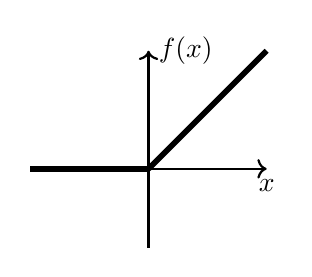
\begin{tikzpicture}
        % Axes
        \draw[thick,->] (-1.5,0) -- (1.5,0) node[anchor=north] {$x$}; % x-axis
        \draw[thick,->] (0,-1) -- (0,1.5) node[anchor=west] {$f(x)$}; % y-axis

        % ReLU function
        \draw[line width=2pt,black] (-1.5, 0) -- (0, 0); % f(x) = 0 for x < 0
        \draw[line width=2pt,black] (0, 0) -- (1.5, 1.5); % f(x) = x for x >= 0
    \end{tikzpicture}
    \captionof{figure}{Rectified linear unit (ReLU)}
  \end{minipage}
  \begin{minipage}[t]{.45\textwidth}
    \centering
    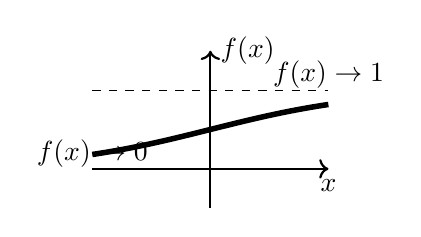
\begin{tikzpicture}
        % Axes
        \draw[thick,->] (-1.5,0) -- (1.5,0) node[anchor=north] {$x$}; % x-axis
        \draw[thick,->] (0,-0.5) -- (0,1.5) node[anchor=west] {$f(x)$}; % y-axis

        % Sigmoid function plot
        \draw[line width=2pt,black,domain=-1.5:1.5,samples=100,smooth] plot (\x, {1/(1 + exp(-\x))});

        % Labels for Sigmoid
        \node at (-1.5, 0.2) {$f(x) \to 0$}; % Description for x -> -∞
        \node at (1.5, 1.2) {$f(x) \to 1$}; % Description for x -> +∞

        % Horizontal lines for asymptotes
        \draw[dashed] (-1.5,1) -- (1.5,1); % y = 1 asymptote
        \draw[dashed] (-1.5,0) -- (1.5,0); % y = 0 asymptote
    \end{tikzpicture}
    \captionof{figure}{Sigmoid activation}
  \end{minipage}
  \caption{Comparison of ReLU and Sigmoid activation functions}
  \label{fig:activation-functions}
\end{figure}


Combining 2 dimensional affine transformation and ReLU gives as the basic Conv2D layer found in most image classification network, like Resnet~\parencite{he2015deepresiduallearningimage} and MobileNet~\parencite{howard2017mobilenetsefficientconvolutionalneural}.
\begin{align}
  ReLU(Conv2D(I, K) + b)
  \label{eq:conv2d}
\end{align}

\section{Layer graphs}
As mentioned, DNNs are neural networks with one or more hidden layers. Generally the amount of layers correlates to better prediction results, due to the increasing amount learnable parameters being able to capture more complex features.

The relationships between layers are presented as graphs, where nodes are layers or fused layers and paths are the data flow directions. Figure~\ref{fig:conv2d-layer} displays the equation~\ref{eq:conv2d} as a simple graph were data flow is always from one layers output to next layers input.

\begin{figure}[ht]
  \centering
  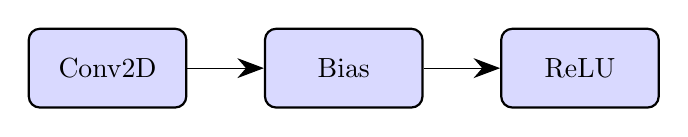
\begin{tikzpicture}
    \node[draw, thick, rectangle, rounded corners, minimum width=2cm, minimum height=1cm, fill=blue!15] (A) at (0,0) {Conv2D};
    \node[draw, thick, rectangle, rounded corners, minimum width=2cm, minimum height=1cm, fill=blue!15] (B) at (3,0) {Bias};
    \node[draw, thick, rectangle, rounded corners, minimum width=2cm, minimum height=1cm, fill=blue!15] (C) at (6,0) {ReLU};

    \path [-{Stealth[scale=2]}] (A) edge node[above] {} (B);
    \path [-{Stealth[scale=2]}] (B) edge node[above] {} (C);
  \end{tikzpicture}
  \caption{Feed forward relationship between Conv2d, bias and ReLU layers.}
  \label{fig:conv2d-layer}
\end{figure}
For clarity this combination of 2D convolution, bias and ReLU is usually fused into single layer node. Different neural network frameworks use slightly different terminology relating to the meaning of operation, layer and fused layer. For example Tensorflow~\cite{tensorflow2015-whitepaper}, a popular framework for training, considers Conv2D, bias and ReLU separate layers and the combination of the a fused layer, where as in Pytorch~\cite{pytorch} the combination of Conv2D, bias and ReLU is considered one layer. For the purposes of this work, we use Tensorflow naming scheme.

The simplest kind of relation is a feedforward relationship where the output of layer A is the input of layer B as shown in the figure~\ref{fig:network-simple}.
Resnet~\cite{he2015deepresiduallearningimage} heavily utilizes what are called residual connections. With residual connection an input of a layer is used in multiple parts of a feed forward network. Figure~\ref{fig:network-residual} shows and example of a residual connection, where input of layer A is used again after concatenation as part of input for layer C.
\begin{figure}
  \centering
  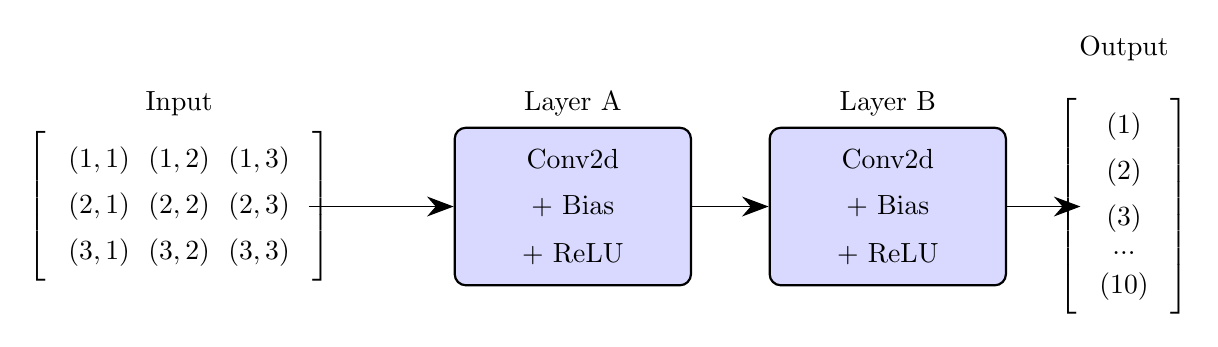
\begin{tikzpicture}
    \node at (-3, 1.3) {Input};
    \matrix [matrix of math nodes, left delimiter={[}, right delimiter={]}, % for the rectangle border
              ampersand replacement=\&] % see explanation
      (mm)
      at(-3, 0)
      {
          \node {(1,1)}; \& \node {(1,2)}; \& \node {(1,3)};\\
          \node {(2,1)}; \& \node {(2,2)}; \& \node {(2,3)};\\
          \node {(3,1)}; \& \node {(3,2)}; \& \node {(3,3)};\\
      };

    % Box A (Layer 1) with sub-nodes Conv2d, Bias, ReLU
    \node[draw, thick, rectangle, rounded corners, minimum width=3cm, minimum height=2cm, fill=blue!15] (A) at (2,0) {};
    \node at (2,1.3) {Layer A}; % Title for Layer 1
    \node at (2,0.6) {Conv2d};
    \node at (2,0) {+ Bias};
    \node at (2,-0.6) {+ ReLU};

    % Box B (Layer 2) with sub-nodes Conv2d, Bias, ReLU
    \node[draw, thick, rectangle, rounded corners, minimum width=3cm, minimum height=2cm, fill=blue!15] (B) at (6,0) {};
    \node at (6,1.3) {Layer B}; % Title for Layer 2
    \node at (6,0.6) {Conv2d};
    \node at (6,0) {+ Bias};
    \node at (6,-0.6) {+ ReLU};

    \node at (9, 2) {Output};
    \matrix [matrix of math nodes, left delimiter={[}, right delimiter={]}, % for the rectangle border
              ampersand replacement=\&] % see explanation
      (out)
      at(9, 0)
      {
          \node {(1)}; \\
          \node {(2)}; \\
          \node {(3)}; \\
          \node {...}; \\
          \node {(10)}; \\
      };

    % Arrow from A to B
    \path [-{Stealth[scale=2]}] (mm) edge node[above] {} (A);
    \path [-{Stealth[scale=2]}] (A) edge node[above] {} (B);
    \path [-{Stealth[scale=2]}] (B) edge node[above] {} (out);
  \end{tikzpicture}
  \caption{Simple feed forward network with two Conv2D with bias and ReLU activation layers.}
  \label{fig:network-simple}
\end{figure}

\begin{figure}
  \centering
    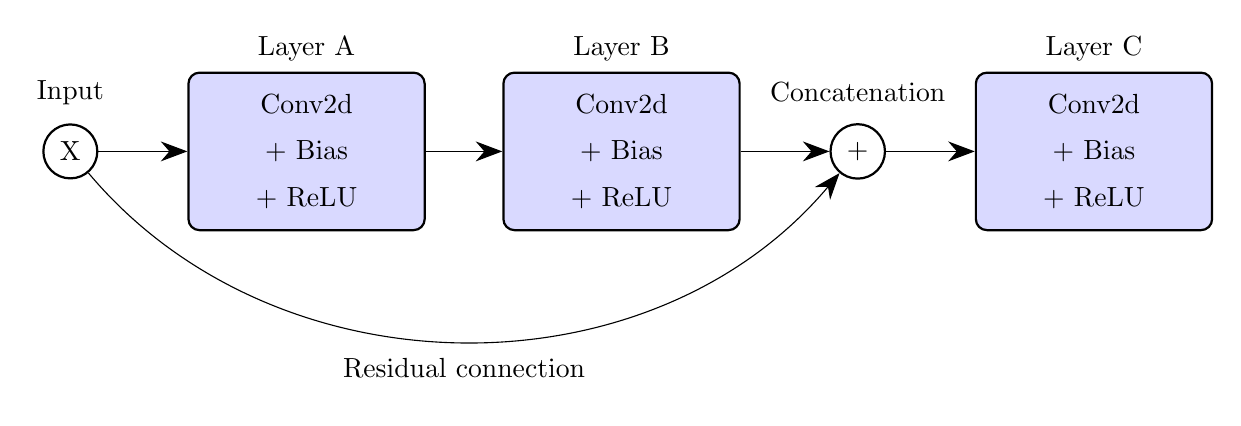
\begin{tikzpicture}
        % Box A (Layer 1) with sub-nodes Conv2d, Bias, ReLU
        \node[draw, thick, rectangle, rounded corners, minimum width=3cm, minimum height=2cm, fill=blue!15] (A) at (0,0) {};
        \node at (0,1.3) {Layer A}; % Title for Layer A
        \node at (0,0.6) {Conv2d};
        \node at (0,0) {+ Bias};
        \node at (0,-0.6) {+ ReLU};

        % Box B (Layer 2) with sub-nodes Conv2d, Bias
        \node[draw, thick, rectangle, rounded corners, minimum width=3cm, minimum height=2cm, fill=blue!15] (B) at (4,0) {};
        \node at (4,1.3) {Layer B}; % Title for Layer B
        \node at (4,0.6) {Conv2d};
        \node at (4,0) {+ Bias};
        \node at (4,-0.6) {+ ReLU};

        % Residual Connection (A to B addition node)
        \node[circle, draw, thick, minimum size=0.6cm] (input) at (-3,0) {X};
        \node[circle, draw, thick, minimum size=0.6cm] (add) at (7,0) {+};
        \node (name1) at (7,0.75) {Concatenation};
        \node (name2) at (2,-2.75) {Residual connection};
        \node (name3) at (-3,0.75) {Input};

        % Arrows from A to B and from B to addition
        %
        \path [-{Stealth[scale=2]}] (input) edge node[above] {} (A);
        \path [-{Stealth[scale=2]}] (A) edge node[above] {} (B);
        \path [-{Stealth[scale=2]}] (B) edge node[above] {} (add);

        % Direct residual connection from A to addition node
        \path [-{Stealth[scale=2]}] (A.east) -- ++(2.5,0) -- (add.west);
        \path [-{Stealth[scale=2]}] (input) edge[bend right=50] node [left] {} (add);

        % Box B (Layer 2) with sub-nodes Conv2d, Bias
        \node[draw, thick, rectangle, rounded corners, minimum width=3cm, minimum height=2cm, fill=blue!15] (C) at (10,0) {};
        \node at (10,1.3) {Layer C}; % Title for Layer B
        \node at (10,0.6) {Conv2d};
        \node at (10,0) {+ Bias};
        \node at (10,-0.6) {+ ReLU};


        \path [-{Stealth[scale=2]}] (add) edge node[above] {} (C);


    \end{tikzpicture}
  \caption{Residual feed forward network with fused layers.}
  \label{fig:network-residual}
\end{figure}


\section{Deep-learning accelerators}
\label{sec:dlas}
In desktop applications and data center workloads neural networks have been accelerated with GPUs, due to their ability to perform linear-algebra operations like matrix multiplication with high amount of parallellity.

In recent times there has been a growing need to also run neural networks in mobile devices. Traditional GPUs are too power-hungry for these small devices, so a need for more efficient accelerators for these workloads has been born. Companies such as Apple and Qualcomm now include multiple mobile DLA's in their SoCs to run applications like face recognition on phones using their chips.

\section{Quantization}
When training DNN models with high level tools like Pytorch, models are built to use floating point operations In recent years big players like NVIDIA have started to utilize more and more quantized integer models. This is due to the fact that as the amount of paramters in models like GPT, has been growing exponentially, there is are significant performance gains available by reducing the granularity of the paramters. Standard floating point value has a width of 32-bits, where as int8 which is the most common integer type in DNNs has just the 8 bits. Thus when less granularity is acceptable similarly performing integer based accelerator can do 4 times the calculations when compared to a floating point accelerator.
Some models reduce that amount of granularity even more and have layers using 4-bit or 2-bit integers. With 2-bit integers one can do 16-times as many calculations in comparison to floating points.

It's also possbile to have only parts of the model quantisized. For these cases it might be necessary to have additional conversion layers to go from floating point inputs to integers and backwards. This can be useful for the cases where the target platform is only able to accelerate quantized layers, but the developer want's to use well proven subnetwork to ensure accuracy while the rest of the network is hardware accelerated to improve performance.

In the case of Headsail's DLA it supports 8-bit, 4-bit and 2-bit integers, with 4-bit and 2-bit inputs using SIMD operations to linearly increase the amount of calculations per cycle.

\section{System-on-chip}
System-on-chips (SoCs) are a form of heterogenous computing, where multiple different computing elements and electronic systems are integrated into one circuit.
SoCs generally include CPUs, memories, IO interfaces and specialized accelerators, but conceptually there is no set definition on what SoC needs to include.
This essentially produces a single functional entity that can easily integrated into multitude of different general processing workloads.
Interconnects between SoC components can be run on very high bitrates, greatly reducing latency.

SoC are often used in mobile devices due to tight integration between components enabling small space footprints, in comparison to separately integrated components.
\fixthis{Coherency means that different components can works on the same data.}
In recent times SoC have also begun being seen more in consumer laptops, effectively handling desktop workloads as is the case with the Apple M-series of chips as well as the Qualcomm Snapdragon Elite X chip, Intel Lunar Lake.

Nowadays SoCs are seen as a solution for the \fixthis{SILICONE APOCALYPSE}, which describes the lessening increase of advance in computational performance of traditional CPUs due to Moore's Law not applying anymore.

\chapter{Methodology}
This section goes over the technologies use to complete this project in detail. First we discuss the hardware used in the SocHub's Headsail SoC and the parts affecting the decision made in the software design in detail. After this we present the used software stack necessary to run neural networks on the described hardware. We will also discuss the virtual prototype on which the majority of the software development took place on, and how it differs from the hardware.
\label{ch:methodology}

\section{Headsail}
Headsail is the third Soc build by the SocHub research group~\parencite{Ballast}. Headsail has two RISCV CPUs, one 32-bit meant for booting up the system called SysCtrl and one 64-bit on called HPC, meant for running the actual applications.
Headsail includes a wide variety of different peripherals, one of which is a custom build the Deep Learning accelerator.

\subsection{DLA}
Headsail's DLA is a MAC array based accelerator, which provides the following operations: Conv2D, Bias, ReLU. The operations are implemented as a pipeline, meaning that the order of operations is always the same. During one layer cycle the operations need to be executed in the following order: Conv2d, Bias, ReLU. This is the most commonly found order in modern neural networks so it suits most use cases. In addition to these operations DLA can perform bit shifting for results of the MAC array and the post-processing pipeline.
Bias and ReLU can be skipped in the case either or both of the aren't needed in the given layer. In this case Conv2D output is used directly and is capped to fit the 8-bit width of the output.
The particular operations are configure from the register interface of the DLA.
DLA has a simple 32 bit RISCV based controller CPU, that can be used to drive the DLA parallel to normal HPC execution, but it's also possible to control the DLA directly from the main CPUs.

\section{TVM}
TVM is a machine learning compiler framework by Apache. Among other features TVM includes, multiple runtimes, accelerator backends, optimizers, and a machine learning library for building and training models. The variety of features allows for TVM to be used to implement a complete machine learning workflow, or TVM can be used to implement part of the workflow with other tools.

TVM has it's own graph representation for neural networks called Relay IR. Like the traditional graph representation Relay IR represents network layers as nodes in a abstract syntax tree, where the data flow of the networks is shown as the relationship between parent and child nodes, where parent nodes output is the input of the child node.

TVM is able to be extended to support additional hardware accelerators by implementing a custom code generation module for the target hardware. In principle the developer defines external C symbols that provide the operation implementations which TVM then injects into the Relay IR models. During runtime TVM then calls these external symbols instead of the default operations provided by the TVM Relay library.

It's possible to generate Relay IR models from other graph formats with TVM. For example common formats like Tensorflow, Torch and Onnx models are officially supported by TVM. This allows developers to build and train their models with tools they might prefer over TVM, and use TVM as a compiler/runtime.

During model compilation TVM is able to optimize the graph and allocate acceleratable nodes to suitable accelerators.~\parencite{TVM}

\subsection{TVM on baremetal}
TVM also provides a tool to run TVM models on baremetal platforms called microTVM. MicroTVM is only dependant on the C standard library and thus can be used in any baremetal system that has a working C-toolchain.

MicroTVM works by generating platform independent C-source code from Relay IR-models, which can then be integrated with the microTVM c-runtime to produce executable binaries to run the network.

With custom codegeneration it's also possible to define baremetal compatible accelerator nodes, which the TVM runtime is able to assign layers for during the C source code generation.~\parencite{TVM}


\section{Renode}
\label{sec:renode}
Renode is a software development framework, which enables developers to use principles of continuous integration when writing hardware dependent code. In essence Renode is a hardware emulator which allows the user to specify exactly which kind of hardware they want to target, down to the implementation of specific peripherals and memory addresses. This streamlines the process of HW/SW integration, since hardware and software can be developed in parallel, which in return reduces the total production time for products.

Renode models a wide variety of different processors and peripherals, but it is also expandable with custom components that are either baked directly into the binary (source code extensions in C\#) or with dynamically loaded python peripherals. Python peripherals are more limited when compared to the C\# peripherals. This project implements the DLA hardware design as a dynamic python peripheral.

While renode is a operation accurate emulator, the Python API isn't. When Renode makes a request to the Python API, it counts as one clock cycle even when realistically the Python API's corresponding hardware implementation would take more than one cycle. The consequence of this that we cannot accurately benchmark DLA in Renode. The benefit of the python API is in rapid development of hardware components.

Since Renode python peripherals don't have a clock, the state of the peripheral can only be changed when a CPU reads or writes to an address that is registered for the peripheral. DLA-VP is designed to run a processing loop after each write to it's memory region. The processing loop checks if the state of DLA-VP is ready for operation execution and if yes performs the operation per configuration. Read accesses don't change the devices internal state, so the processing loop isn't executed on them. After the executing write call, the result of the operation can be read on the next clock cycle from the peripherals memory region.

\chapter{Implementation}
\label{ch:implementation}
This section covers the actual implementation of the used software stack in detail and the specific use cases developed on top of the stack. As well as the TinyPerf benchmark used to evaluate the performnace of the DLA.

\section{Software support}
\label{sec:software_support}
Even though Headsail is the third SoCHub Soc, it had little existing software support for C. Previous SoCs had only support for Riscv-rt in rust. So a major part of this project involved setting up a Headsail compatible C toolchain. Since Headsail has RISCV CPUs we could use an already existing riscv-gnu-toolchain for the compiler, but we still had to set up a C standard library for the chip with custom version of newlib libgloss. Also due to specific memory addressing decisions in the hardware, we needed to use medany code model compatible compiler and standard library when targeting the 64-bit processor.

We also developed a Board Support Package for Headsail, which provides drivers for the different peripherals in the SoC. Most importantly for this project, the driver for the DLA is included in the BSP.
The DLA driver is implemented in two layers. First is the low level layer which implements functions that directly target the register interface in the DLA to drive the hardware. The second is the high level layer which abstracts the low level layer to provied simple calls for the 3 different DLA operations. The high level layer also provides the external symbols for DLA operations used by the TVM code generation.

Headsail-BSP is written in Rust, so to use it with the C based TVM code we also needed to provide a Foreign Function Interface.


\section{Porting Newlib}
Newlib is an implementation of the C standard library meant for use in embedded devices~\parencite{newlib}. We chose to use Newlib for our C standard library in Headsail since it's known to be relatively easy to port for new platforms. Newlib is separated into two different parts. First is the Newlib core which implements the actual standard library for different CPU ISA's. Since Newlib already has support for RISCV we didn't need to modify Newlib core in anyway. Second part of Newlib is called Libgloss, which implements the platform dependant features. Since Headsail is a custom platform we needed to implement most of the libgloss for it from scratch.

Porting libgloss involves implementing 16 syscalls, CRT0 and a linker script. From the 16 syscalls only some are mandatory for us to implement, because we are targeting bare-metal applications. The table~\ref{tab:newlib_syscalls} shows all the libgloss syscalls with column 3 displaying if we implemented the call. The unimplemented calls still need to be defined in the libgloss source for linking purposes but they don't need do anything except return an error. For example the fork syscall duplicates a process, but since we don't support multithreading or any other form of process concurrency it will never be called, thus having it return error is correct.

\begin{lstlisting}[language=C, caption={Minimal implmentation of the fork() syscall in Newlib Libgloss}]
  int _fork() {
      return -1;
  }
\end{lstlisting}

The system calls can be implemented either in non-reentrant or reentrant way. Reentrant system calls are thread safe but require an additional argument, reentrancy structure, to be passed. Reentrancy strucutre holds local values specific for that instance of the function call, where as the non-reentrant version of the function refers to shared global variables. For single threaded applications on headsail implementing the non-reentrant systems calls was enough.~\parencite{bennett2010porting}


\begin{table}[htbp]
\centering
\begin{tabular}{|l|l|c|}
\hline
\textbf{Syscall}       & \textbf{Description}               & \textbf{Implemented (Bool)} \\ \hline
\texttt{exit}         & Terminates the process             & Yes                       \\ \hline
\texttt{close}         & Closes a file                      & No                       \\ \hline
\texttt{fstat}         & Gets file status                   & Yes                       \\ \hline
\texttt{getpid}        & Gets the process ID                & No                       \\ \hline
\texttt{isatty}        & Tests if a file descriptor is a terminal & Yes                 \\ \hline
\texttt{kill}          & Removes a process                    & No                       \\ \hline
\texttt{link}          & Creates a hard link to a file      & No                       \\ \hline
\texttt{lseek}         & Re-positions read/write file offset & No                       \\ \hline
\texttt{open}          & Opens a file                       & No                       \\ \hline
\texttt{read}          & Reads from a file                  & Yes                       \\ \hline
\texttt{sbrk}          & Moves end of heap pointer          & Yes                       \\ \hline
\texttt{stat}          & Retrieves file status              & No                       \\ \hline
\texttt{times}         & Returns process times              & No                       \\ \hline
\texttt{unlink}        & Deletes a name or a file           & No                       \\ \hline
\texttt{wait}          & Waits for process to change state  & No                       \\ \hline
\texttt{write}         & Writes to a file                   & Yes                       \\ \hline
\end{tabular}
\caption{Newlib Syscalls and Implementation Status}
\label{tab:newlib_syscalls}
\end{table}


\section{DLA Software Architecture}
The figure~\ref{fig:architecture} shows the high level software architecture of TVM annotated model deployment flow with Headsail DLA. First we use high level operations in DLA driver to provied external symbols for Conv2d, Bias and ReLU. These are referenced in the Headsail build of TVM dylib when built with the Headsail custom code generation option.

In other branch we train and optimize a quantisized convolutional neural network with Pytorch and convert the produced model into a ONNX graph.
We then use a python script to load in the Headsail TVM dylib which is used to generate C source code for the model from the annoteted ONNX graph. This code now includes calls to the DLA driver operations.

Finally we produce an executable binary by combining the microTVM C runtime from the Headsail TVM build, generated C source code for the model, Headsail-bsp for the board functions, Headsail-newlib for the C standard library and finally the use case program.

\begin{figure}
  \centering
  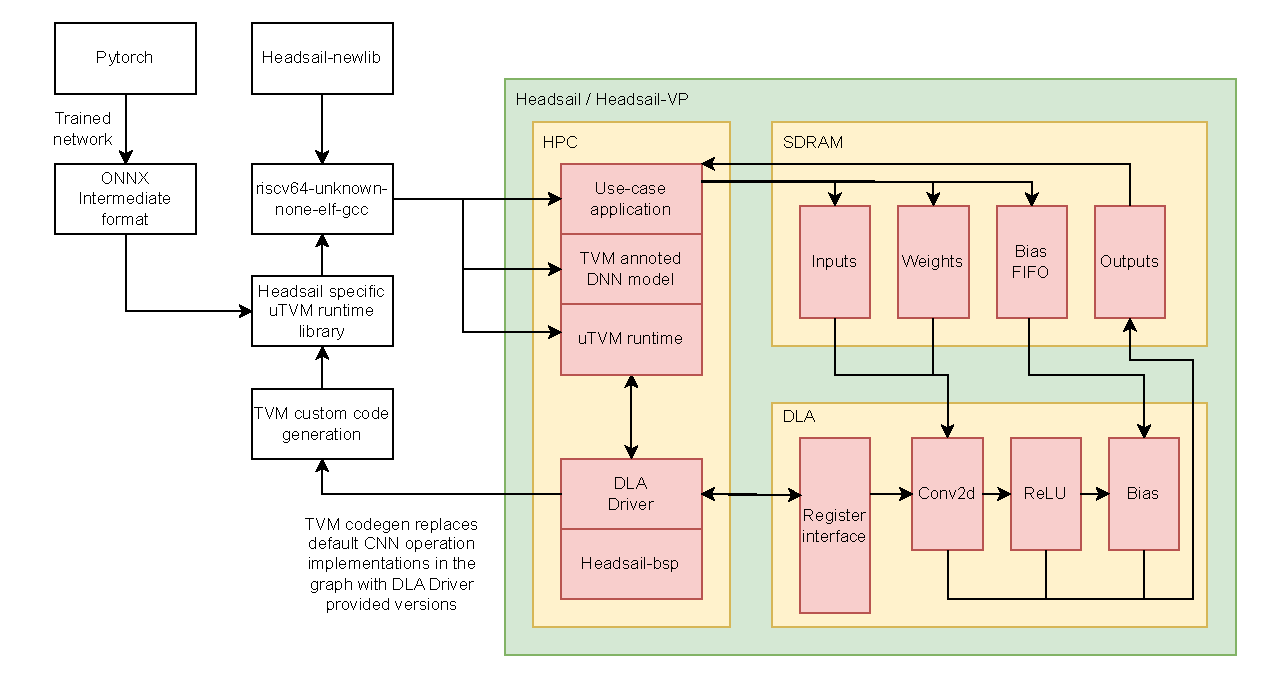
\includegraphics[width=\textwidth]{img/dla-architecture.pdf}
  \caption{Architecture of accelerated DLA flow in Headsail with TVM runtime and a Pytorch model}
  \label{fig:architecture}
\end{figure}


\section{Benchmarking}
For the DLA there are two things we can benchmark. First is to look at the amount of convolution operations we can execute per time unit. This kind of throughput benchmarking fine but doesn't tell us much about the real-life CNN performance, since it doesn't take in to account what proportion of the CNN workloads is actually Conv2d and the proceeding Bias and ReLU operations.

For this reason we need to also do benchmarks with actual CNNs. For this purpose we use MLPerf Tiny Benchmark from MLCommons, which is a benchmarking suite for benchmarking ML inference in low power targets, like MCUs with Deep Learning Accelerators.~\parencite{tinyperf}

TinyPerf consits of four benchmarks meant to target different use cases shown in table~\ref{tab:tinyperf}. From these benchmarks the Anomaly Detection is unacceleratable with the Headsail DLA since it uses FC-AutoEncoder network, which is based on fully connected layers and thus has no operations which our accelerator can execute.

\begin{table}[ht]
\centering
\caption{Tiny Performance Benchmarks, from~\parencite{tinyperf}}
\begin{adjustbox}{max width=\textwidth}
\begin{tabular}{lccc}
    \toprule
    \textbf{Benchmark} & \textbf{Dataset (Input Size)} & \textbf{Model (TFLite Model Size)} & \textbf{Quality Target (Metric)} \\
    \midrule
    Keyword Spotting & Speech Commands (49x10) & DS-CNN (52.5 KB) & 90\% (Top-1) \\
    Visual Wake Words & VWW Dataset (96x96)  & MobileNetV1 (325 KB) & 80\% (Top-1) \\
    Image Classification & CIFAR10 (32x32) & ResNet (96 KB) & 85\% (Top-1) \\
    Anomaly Detection & ToyADMOS (5x128)  & FC-AutoEncoder (270 KB) & .85 (AUC) \\
    \bottomrule
\end{tabular}
\end{adjustbox}
\label{tab:tinyperf}
\end{table}

\chapter{Conclusions}
\label{ch:conclusions}©@
%
% The bibliography, i.e the list of references
%
\newpage

\printbibliography[title=References]
\addcontentsline{toc}{chapter}{References}


%
% Appendices are optional. 
% This part is semi-ugly at the moment. Please give feedback if can
% improve it.

\appendix
\pagestyle{headings}



%
% a) Not-so-handy way, but at least it works
% 
\def\appA{APPENDIX A. Something extra} % Define the name and numbering manually
\chapter*{\appA}                       % Create chapter heading
\markboth{\appA}{\appA}                % Set page header
\addcontentsline{toc}{chapter}{\appA}  % Include this in TOC
% Note that \label does not work with unnumbered chapter

Appendices are purely optional.  All appendices must be referred to in
the body text

\def\appB{APPENDIX B. Something completely different} % Define another new command
\chapter*{\appB}                       % As above, but use \appB instead of \appA
\label{app:B}
\markboth{\appB}{\appB}                     
\addcontentsline{toc}{chapter}{\appB}  


You can append to your thesis, for example, lengthy mathematical
derivations, an important algorithm in a programming language, input
and output listings, an extract of a standard relating to your thesis,
a user manual, empirical knowledge produced while preparing the
thesis, the results of a survey, lists, pictures, drawings, maps,
complex charts (conceptual schema, circuit diagrams, structure charts)
and so on.


%
% b) The other option is to use numbered chapter and our baseline
% template report.cls numbers them as A, B... The heading and TOC do
% not include prefix 'Appendix' although the page header does.
%\chapter{name of the appendix}
%\label{app:A}                          % For cross-references



\end{document}


% LocalWords:  quantizising
